\hl{Your appendies goes here.}
~\\
~\\
~\\

\begin{table}
	\begin{tabular}{ |p{3cm}||p{3cm}|p{3cm}|p{3cm}|  }
		\hline
		\multicolumn{4}{|c|}{Country List} \\
		\hline
		Country Name     or Area Name& ISO ALPHA 2 Code &ISO ALPHA 3 Code&ISO numeric Code\\
		\hline
		Afghanistan   & AF    &AFG&   004\\
		Aland Islands&   AX  & ALA   &248\\
		Albania &AL & ALB&  008\\
		Algeria    &DZ & DZA&  012\\
		American Samoa&   AS  & ASM&016\\
		Andorra& AD  & AND   &020\\
		Angola& AO  & AGO&024\\
		\hline
	\end{tabular}
	\caption{\hl{Title of the table}}
\end{table}



\begin{figure}[!t]
	\label{figSTRCT}
	\caption{\hl{Title of the figure}}
	\begin{center}
		\setlength\fboxsep{0.3pt}
		\setlength\fboxrule{0.4pt}
		\fbox{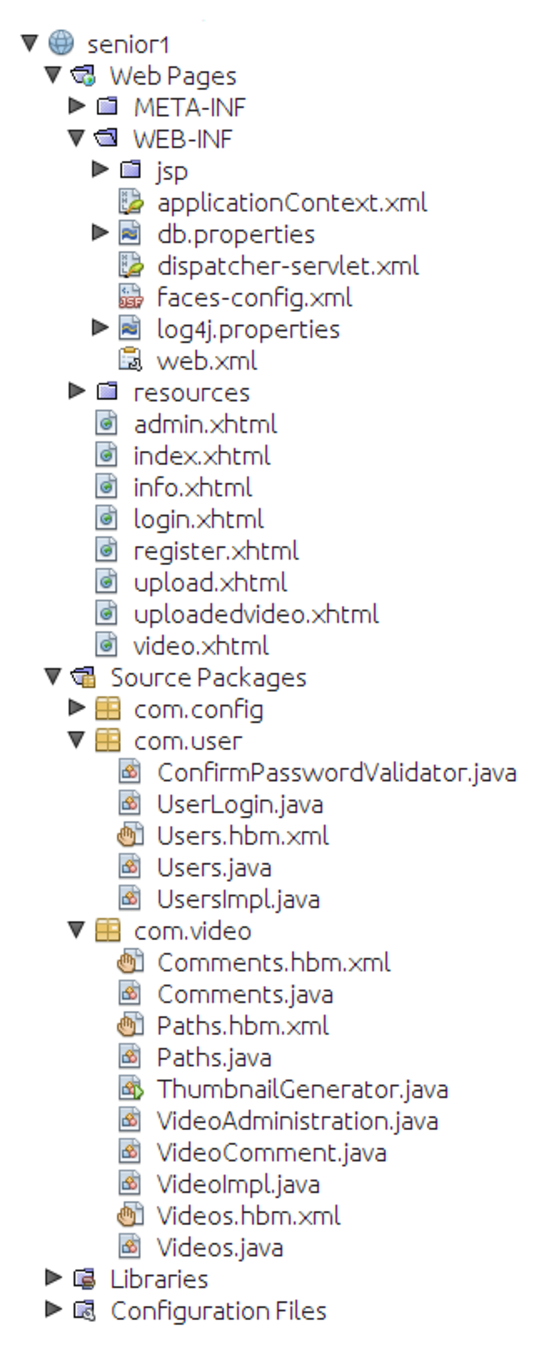
\includegraphics[scale=0.57]{picture/project_structure}}
	\end{center}
\end{figure}



\begin{algorithm}[H]
	\KwData{this text}
	\KwResult{how to write algorithm with \LaTeX2e }
	initialization\;
	\While{not at end of this document}{
	 read current\;
	 \eIf{understand}{
	  go to next section\;
	  current section becomes this one\;
	  }{
	  go back to the beginning of current section\;
	 }
	}
	\caption{\hl{Title of the Algorithm}}
\end{algorithm}


\newpage
\begin{code}
	\lstinputlisting[label=samplecode1,language=java, firstline=1, lastline=40]{project/src/java/com/user/UserLogin.java}
	\caption{\hl{Title of Code 1}}
\end{code}

\newpage
\begin{code}
	\lstinputlisting[label=samplecode2,language=xml]{project/src/java/com/user/Users.hbm.xml}
	\caption{\hl{Title of Code 2}}
\end{code}

\newpage
\begin{code}
	\lstinputlisting[label=samplecode3,language=html]{project/web/uploadedvideo.xhtml}
	\caption{\hl{Title of Code 3}}
\end{code}



\ac{ECC} is an acronym.




